\chapter{Mesure du temps d'exécution des 20 nombres premiers ayant la meme taille}
\section{Experimentation}
Le tableau suivant représente les temps d'exécution en nanoseconde de l'algorithme selon la variation des nombres premiers x1..x2 en ordre croissante.\\ \\
\par
\small
\resizebox{17cm}{!}{
\begin{tabular}{| c | c | c | c | c | c | c | c | c | c | c |}
    \hline
     x1 & x2 & x3 & x4 & x5 & x6 & x7 & x8 & x9 & x10   \\
    \hline
   1500450271 &
18790481837&
1979339339&
2030444287&
2860486313&
3267000013&
3367900313&
3628273133&
4093082899 & 4392489041\\
    \hline
    
     x11 & x12 & x13 & x14 & x15 & x16 & x17 & x18 & x19 & x20   \\
    \hline
    5038465463&
5463458053&
5555333227&
5754853343&
5915587277&
6668999101&
7896879971&
8278487999&
9471413089&
9576890767 \\
    \hline
\end{tabular}}
\\ \\
\par
\small
\resizebox{17cm}{!}{
\begin{tabular}{| c | c | c | c | c | c | c | c | c | c | c |}
    \hline
    x &  x1 & x2 & x3 & x4 & x5 & x6 & x7 & x8 & x9 & x10   \\
    \hline
    A1(s) & 16.113 &
20.109 &
19.987&
20.75&
44.815&
59.697&
48.246&
55.874&
68.331&
70.699
 \\
    \hline
    A2(s) & 8.206 &
9.687&
10.146&
15.69&
26.938&
28.324&
24.693&
31.044&
37.252&
34.662 \\
    \hline
    A3(s) &  0.002&
0.001&
0.001&
0.001&
0.001&
0.001&
0.001&
0.001&
0&
0.001\\
    \hline
    A4(s) & 8.198 &
10.035&
13.046&
17.019&
14.282&
20.343&
20.192&
22.26&
22.948&
25.089 \\
    \hline
    A5(s) & 4.429 &
5.178&
5.594&
5.062&
7.355&
8.195&
8.504&
9.544&
10.064&
11.134 \\
    \hline
    A6(s) & 0 &
0&
0&
0&
0.001&
0.001&
0.001&
0.001&
0.001&
0.001 \\
    \hline
\end{tabular}}
\\ \\
\par
\small
\resizebox{17cm}{!}{
\begin{tabular}{| c | c | c | c | c | c | c | c | c | c | c |}
    \hline
     &  x11 & x12 & x13 & x14 & x15 & x16 & x17 & x18 & x19 & x20   \\
    \hline
    A1(s) & 85.505&
59.221&
84.891&
68.61&
89.415&
94.345&
97.925&
93.204&
114.139&
152.4 \\
    \hline
    A2(s) & 28.492 &
48.4&
48.453&
50.096&
38.766&
34.916&
42.29&
48.979&
56.765&
106.045 \\
    \hline
    A3(s) & 0.002 &
0.001&
0.002&
0.001&
0.001&
0.002&
0.004&
0.004&
0.003&
0.002 \\
    \hline
    A4(s) & 29.859 &
34.864&
35.669&
34.387&
33.805&
36.295&
44.952&
44.042&
51.325&
52.909 \\
    \hline
    A5(s) & 12.632 &
13.641&
14.342&
14.516&
14.809&
20.352&
21.77&
21.964&
26.168&
24.905 \\
    \hline
    A6(s) &0.001&
0.001&
0&
0.001&
0.002&
0.001&
0.001&
0&
0.001&
0.001 \\
    \hline
\end{tabular}}
\\

\normalsize
\par
La figure suivante (voir Figure \ref{fig:chart}) représente l'évolution du temps d'exécution selon l'algorithme utilisee.

\begin{figure}[H]
    \centering
        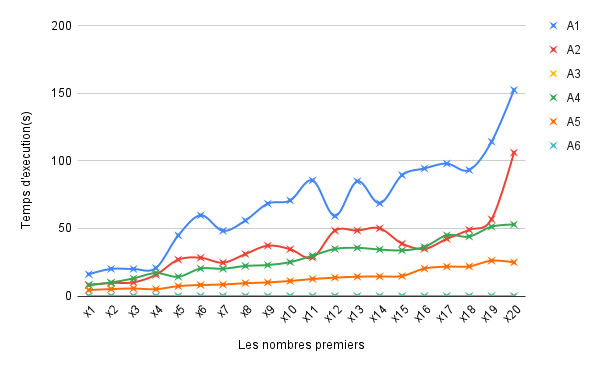
\includegraphics[scale=0.7]{chart.png}
        \caption{Temps d'exécution du programme selon l'algorithme utilisee}
    \label{fig:chart}
\end{figure}
\par
Depuis le graphe, les courbes  sont sous forme des arcs ascendants, on observe que le temps d’exécution évolue de manière presque linéarithmique avec l’augmentation des nombres premiers , avec A6 et A3 comme des meilleurs temps d'execution qui correspond bien à la complexité théorique calculée auparavant , On a pas obtenu une droite linéaire
car les testes étaient peu et aléatoires.

\section{Conclusion}
Les algorithmes A6 , A3 proposent une complexite optimale pour les tests de primalites quelque soit la taille de nombre. et pour ameliorer les resultats on veut tester les algorithmes plusieurs fois ce qu'on va voir dans le chapitre suivant .